\documentclass[tikz,border=10pt]{standalone}
\usepackage{tikz}
\usetikzlibrary{shapes, arrows.meta, calc, backgrounds, positioning, patterns, shadows}

% -------- PALETTE COLORI --------
% 1. Famiglia L^p (FREDDI)
\definecolor{L1loc}{RGB}{215, 235, 250}
\definecolor{L1col}{RGB}{130, 190, 255}
\definecolor{L2col}{RGB}{100, 160, 240}
\definecolor{Linfcol}{RGB}{70, 130, 200}

% 2. Famiglia H^s (VIOLA - SOBOLEV)
\definecolor{H1col}{RGB}{210, 160, 240}   % Lilla
\definecolor{Hscol}{RGB}{160, 100, 220}   % Viola
\definecolor{Hnegcol}{RGB}{140, 90, 180}  % Indaco (Dual)

% 3. Famiglia C^k (CALDI)
\definecolor{C0col}{RGB}{255, 240, 200}
\definecolor{C1col}{RGB}{255, 215, 160}
\definecolor{Ckcol}{RGB}{250, 190, 120}
\definecolor{Cinfcol}{RGB}{240, 160, 100}

% 4. Distribuzioni
\definecolor{Scol}{RGB}{255, 200, 220}
\definecolor{Sprimecol}{RGB}{230, 210, 230}
\definecolor{Eprimecol}{RGB}{200, 230, 180}

% 5. Speciali
\definecolor{C0infcol}{RGB}{255, 255, 150}
\definecolor{Deltacol}{RGB}{220, 80, 80}

% Sfondo
\definecolor{Bgcol}{RGB}{250, 250, 250}
\definecolor{Bgdraw}{RGB}{180, 180, 180}

\begin{document}

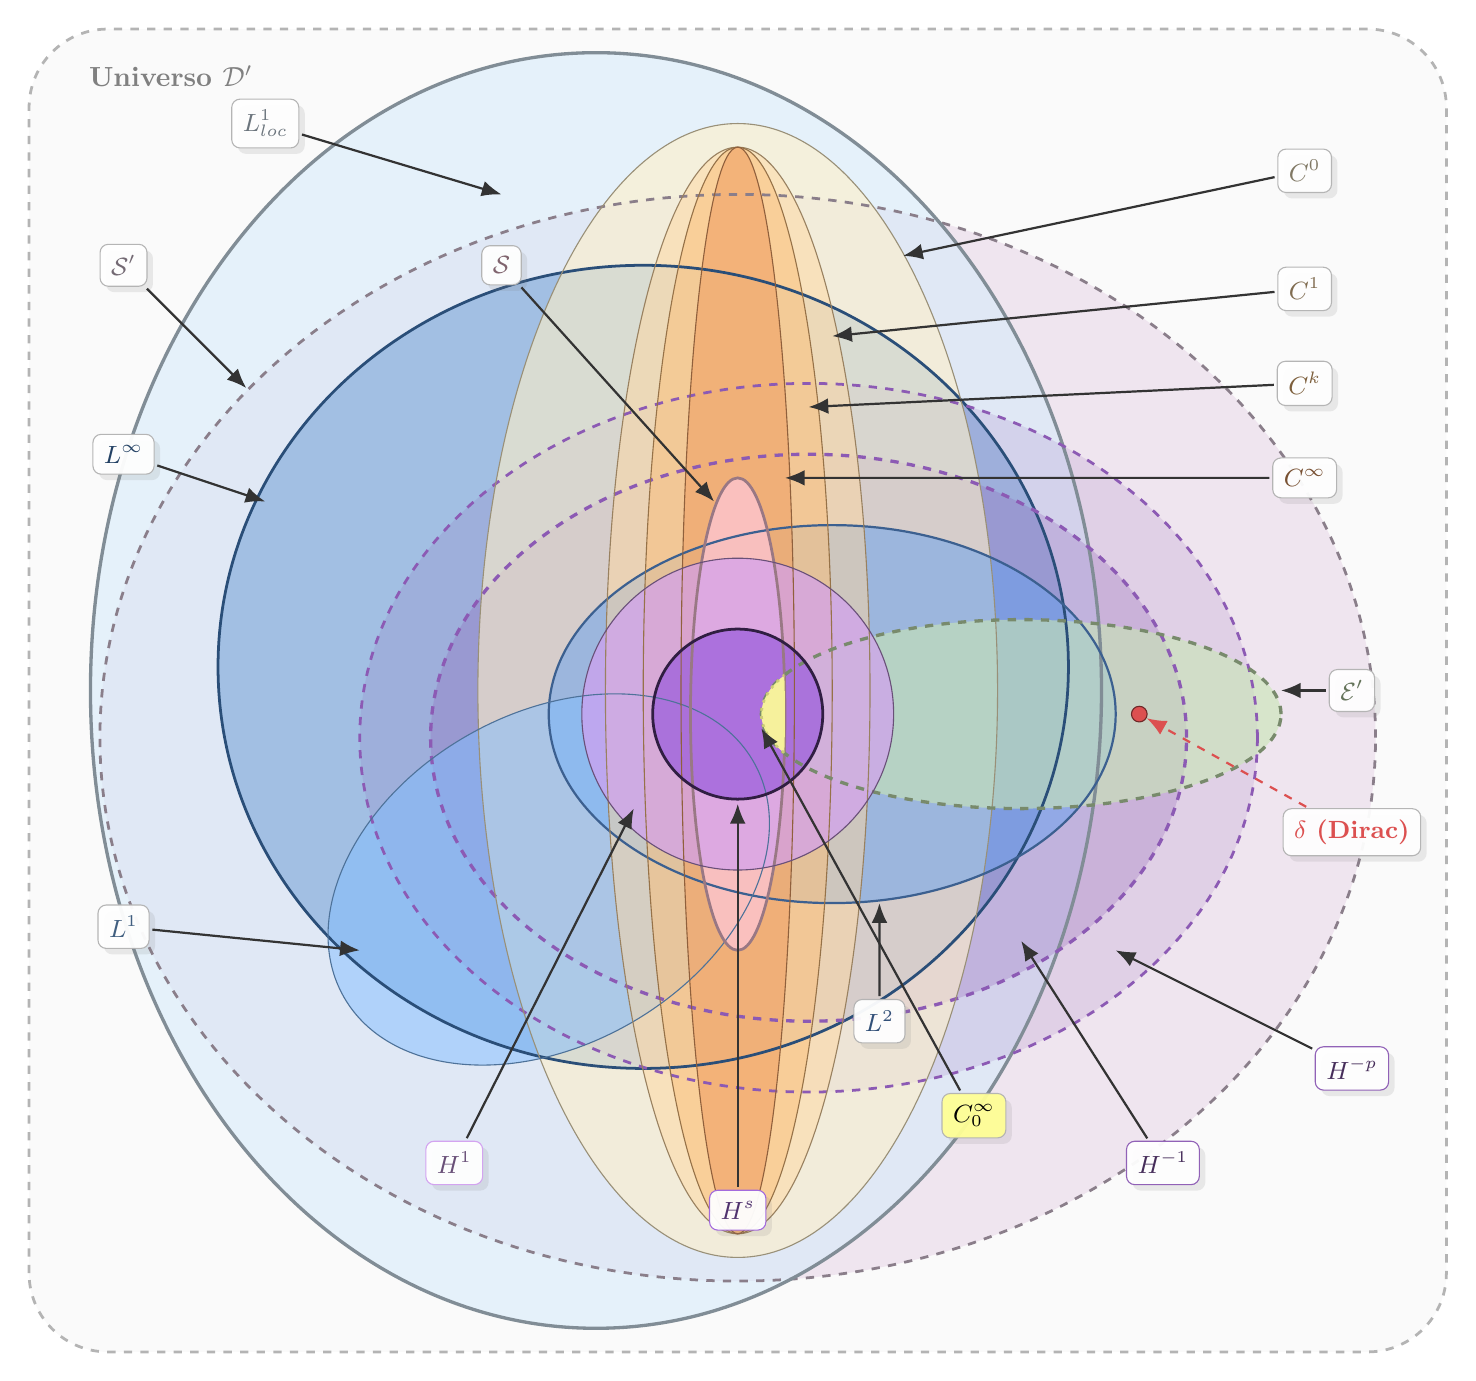
\begin{tikzpicture}[
    scale=0.6, 
    every node/.style={align=center},
    labelbox/.style={
        rectangle, rounded corners=3pt,
        draw=black!30, fill=white,
        inner sep=4pt, font=\small\bfseries,
        drop shadow={opacity=0.15},
        opacity=0.95, text opacity=1
    },
    arrowstyle/.style={
        -{Latex[length=2.5mm, width=2mm]}, 
        line width=0.8pt,
        color=black!80,
        shorten >=0pt, shorten <=1pt 
    }
]

    % Definizioni forme
    \def\pathS{(0,-0.5) ellipse (1.0 and 5.0)}
    \def\pathEprime{(6,-0.5) ellipse (5.5 and 2.0)} 

    % ------------------- RIEMPIMENTI -------------------

    % Universo D'
    \fill[Bgcol, rounded corners=1cm] (-15,-14) rectangle (15,14);

    % S' (Distribuzioni Temperate)
    \fill[Sprimecol, opacity=0.5] (0,-1) ellipse (13.5 and 11.5);

    % L^1_loc (IL GRANDE CONTENITORE DI FUNZIONI)
    % Deve contenere C0 (h=12) e L^inf. Deve fermarsi prima della delta (x=8).
    % Centro: (-3, 0). Raggio X: 10.5 (arriva a 7.5). Raggio Y: 13.5 (copre tutto).
    \fill[L1loc, opacity=0.6] (-3,0) ellipse (10.7 and 13.5);

    % L^inf (Contenuto in L1loc)
    \fill[Linfcol, opacity=0.4] (-2, 0.5) ellipse (9.0 and 8.5);

    % H negativi (Distribuzioni - escono da L1loc a destra)
    \fill[Hnegcol, opacity=0.15] (1.5,-1.0) ellipse (9.5 and 7.5); % H^-p
    \fill[Hnegcol, opacity=0.25] (1.5,-1.0) ellipse (8.0 and 6.0); % H^-1

    % C^0 (Contenuto in L1loc)
    \fill[C0col, opacity=0.6] (0,0) ellipse (5.5 and 12);

    % L^2
    \fill[L2col, opacity=0.5] (2.0,-0.5) ellipse (6.0 and 4.0);

    % L^1
    \fill[L1col, opacity=0.5, rotate around={30:(-4,-4)}] (-4,-4) ellipse (5 and 3.5);

    % Famiglia C nested
    \fill[C1col, opacity=0.5] (0,0) ellipse (2.8 and 11.5);
    \fill[Ckcol, opacity=0.5] (0,0) ellipse (2.0 and 11.5);
    \fill[Cinfcol, opacity=0.6] (0,0) ellipse (1.2 and 11.5);

    % S
    \fill[Scol, opacity=0.7] \pathS;
    
    % E'
    \fill[Eprimecol, opacity=0.6] \pathEprime;

    % H positivi
    \fill[H1col, opacity=0.7] (0,-0.5) circle (3.3);
    \fill[Hscol, opacity=0.8] (0,-0.5) circle (1.8);

    % ------------------- BORDI -------------------

    % D' -> Dashed
    \draw[Bgdraw, dashed, line width=1pt, rounded corners=1cm] (-15,-14) rectangle (15,14);
    
    % S' -> Dashed
    \draw[Sprimecol!60!black, dashed, line width=1pt] (0,-1) ellipse (13.5 and 11.5);
    
    % L1 loc (Funzioni) -> SOLID
    % Ora include visivamente tutto ciò che è funzione classica
    \draw[L1loc!60!black, line width=1.2pt] (-3,0) ellipse (10.7 and 13.5);
    
    % L^inf (Funzioni) -> Solid
    \draw[Linfcol!60!black, line width=1pt] (-2, 0.5) ellipse (9.0 and 8.5);

    % H negativi (Distribuzioni) -> Dashed
    \draw[Hnegcol, dashed, line width=1pt] (1.5,-1.0) ellipse (9.5 and 7.5);
    \draw[Hnegcol, dashed, line width=1.2pt] (1.5,-1.0) ellipse (8.0 and 6.0);

    % C^0 -> Solid
    \draw[C0col!60!black] (0,0) ellipse (5.5 and 12);
    
    % L^2 -> Solid
    \draw[L2col!60!black, line width=0.8pt] (2.0,-0.5) ellipse (6.0 and 4.0);
    
    % L^1 -> Solid
    \draw[L1col!60!black, rotate around={30:(-4,-4)}] (-4,-4) ellipse (5 and 3.5);

    % C^k -> Solid
    \draw[C1col!60!black] (0,0) ellipse (2.8 and 11.5);
    \draw[Ckcol!60!black] (0,0) ellipse (2.0 and 11.5);
    \draw[Cinfcol!60!black] (0,0) ellipse (1.2 and 11.5);
    
    % S -> Solid
    \draw[Scol!60!black, line width=1pt] \pathS;
    
    % E' -> Dashed
    \draw[Eprimecol!60!black, dashed, line width=1.2pt] \pathEprime;

    % Cuore C0inf
    \begin{scope}
        \clip \pathS;
        \fill[C0infcol, opacity=0.9] \pathEprime;
        \draw[C0infcol!80!black, dotted, line width=1pt] \pathEprime;
    \end{scope}

    % H positivi -> Solid
    \draw[H1col!50!black] (0,-0.5) circle (3.3);
    \draw[Hscol!30!black, line width=1pt] (0,-0.5) circle (1.8);

    % ------------------- PUNTO DELTA (Dirac) -------------------
    % Coordinate: x=8.0 (Fuori da L1loc che finisce a 7.5)
    \node[circle, fill=Deltacol, inner sep=2pt, draw=Deltacol!50!black] (ptDelta) at (8.5, -0.5) {};

    % ------------------- LABELS -------------------

    % --- SINISTRA ALTO ---
    \node[text=gray, font=\bfseries] at (-12, 13) {Universo $\mathcal{D}'$};
    
    \node[labelbox, text=Sprimecol!50!black] (lSprime) at (-13, 9) {$\mathcal{S}'$};
    \draw[arrowstyle] (lSprime) -- (-10.4, 6.4);
    
    % L1loc: Spostato in alto per indicare il Grande Contenitore
    \node[labelbox, text=L1loc!50!black] (lL1loc) at (-10, 12) {$L^1_{loc}$};
    \draw[arrowstyle] (lL1loc) -- (-5, 10.5); % Punta al bordo alto di L1loc
    
    % L^inf
    \node[labelbox, text=Linfcol!50!black] (lLinf) at (-13, 5) {$L^\infty$};
    \draw[arrowstyle] (lLinf) -- (-10.0, 4.0);
    
    % --- SINISTRA BASSO ---
    \node[labelbox, text=L1col!50!black] (lL1) at (-13, -5) {$L^1$};
    \draw[arrowstyle] (lL1) -- (-8, -5.5);

    % --- DESTRA ALTO ---
    \node[labelbox, text=C0col!50!black] (lC0) at (12, 11) {$C^0$};
    \draw[arrowstyle] (lC0) -- (3.5, 9.2);

    \node[labelbox, text=C1col!50!black] (lC1) at (12, 8.5) {$C^1$};
    \draw[arrowstyle] (lC1) -- (2.0, 7.5);

    \node[labelbox, text=Ckcol!50!black] (lCk) at (12, 6.5) {$C^k$};
    \draw[arrowstyle] (lCk) -- (1.5, 6);

    \node[labelbox, text=Cinfcol!50!black] (lCinf) at (12, 4.5) {$C^\infty$};
    \draw[arrowstyle] (lCinf) -- (1.0, 4.5);

    % --- DESTRA BASSO ---
    \node[labelbox, text=Eprimecol!50!black] (lEprime) at (13, 0) {$\mathcal{E}'$};
    \draw[arrowstyle] (lEprime) -- (11.5, 0);

    \node[labelbox, text=Deltacol] (lDelta) at (13, -3) {$\delta$ (Dirac)};
    \draw[arrowstyle, dashed, color=Deltacol] (lDelta) -- (ptDelta); 

    \node[labelbox, draw=Hnegcol, text=Hnegcol!50!black] (lHnegP) at (13, -8) {$H^{-p}$};
    \draw[arrowstyle] (lHnegP) -- (8.0, -5.5);

    \node[labelbox, draw=Hnegcol, text=Hnegcol!50!black] (lHneg1) at (9, -10) {$H^{-1}$};
    \draw[arrowstyle] (lHneg1) -- (6.0, -5.3);

    % --- CENTRO ---
    \node[labelbox, text=Scol!50!black] (lS) at (-5, 9) {$\mathcal{S}$};
    \draw[arrowstyle] (lS) -- (-0.5, 4);

    \node[labelbox, fill=C0infcol, text=black] (lC0inf) at (5, -9) {$C_0^\infty$};
    \draw[arrowstyle] (lC0inf) -- (0.5, -0.8);

    % --- CENTRO BASSO ---
    \node[labelbox, text=L2col!50!black] (lL2) at (3, -7) {$L^2$};
    \draw[arrowstyle] (lL2) -- (3.0, -4.5);

    \node[labelbox, draw=H1col, text=H1col!50!black] (lH1) at (-6, -10) {$H^1$};
    \draw[arrowstyle] (lH1) -- (-2.2, -2.5);

    \node[labelbox, draw=Hscol, text=Hscol!50!black, font=\small\bfseries] (lHs) at (0, -11) {$H^s$};
    \draw[arrowstyle] (lHs) -- (0, -2.4);

\end{tikzpicture}
\end{document}